\section{Поверхностные интегралы}
\subsection{Поверхности}
\begin{note}(от редактора)
В данном параграфе не следует путать топологическое определение границы множества $\partial S = \overline{S} \setminus \text{int}(S)$ и понятие края (в смысле дифференциальной геометрии), которое определяется для поверхностей. Точка $p\in S$ принадлежит краю, если её окрестность в $S$ (как в двумерной поверхности) "обрывается". К сожалению край обозначается также $\partial S$ и понять где-что можно только из контекста. В этом параграфе будет только край. Рассмотрим разницу на примере, у сферы границей является вся сфера, а края нет, но вот у полусферы уже есть край --- это ее экватор.
\end{note}

\begin{reminder}
\hypertarget{homeomorphism_definition}{}
Будем говорить, что $F \in C(\Omega, \R^m)$, где $\Omega \subset \R^m$, является гомеоморфизмом, если $\exists F^{-1}$: $F(\Omega) \mapsto \Omega$, такое что $F^{-1} \in C(F(\Omega), \Omega)$.
\end{reminder}

\begin{reminder}
    Множество $G \in R^n$ называется областью, если:
\begin{itemize}
    \item $G$ является открытым множеством.
    \item $G$ является связным множеством (любые две точки из $G$ можно соединить непрерывной кривой, целиком лежащей в $G$).
\end{itemize}
\end{reminder}

\noindent 
\begin{minipage}{0.55\textwidth}
\begin{definition}
    Пусть $G \subset \R^2_{uv}$~---~область. Пусть $\overline{r}: \overline{G} \rightarrow \R^3$, $\overline{r} \in C(\overline{G}, \R^3)$ и $\overline{r}$~---~гомеоморфизм на $G$. Тогда будем называть:
    \begin{enumerate}
        \item[$\bullet$] $S := \overline{r}(\overline{G})$~---~\textit{поверхностью};
        \item[$\bullet$] $\partial  S := \overline{r}(\partial G)$~---~\textit{краем} этой поверхности.
    \end{enumerate}
\end{definition}
\end{minipage}
\begin{minipage}{0.45\textwidth}
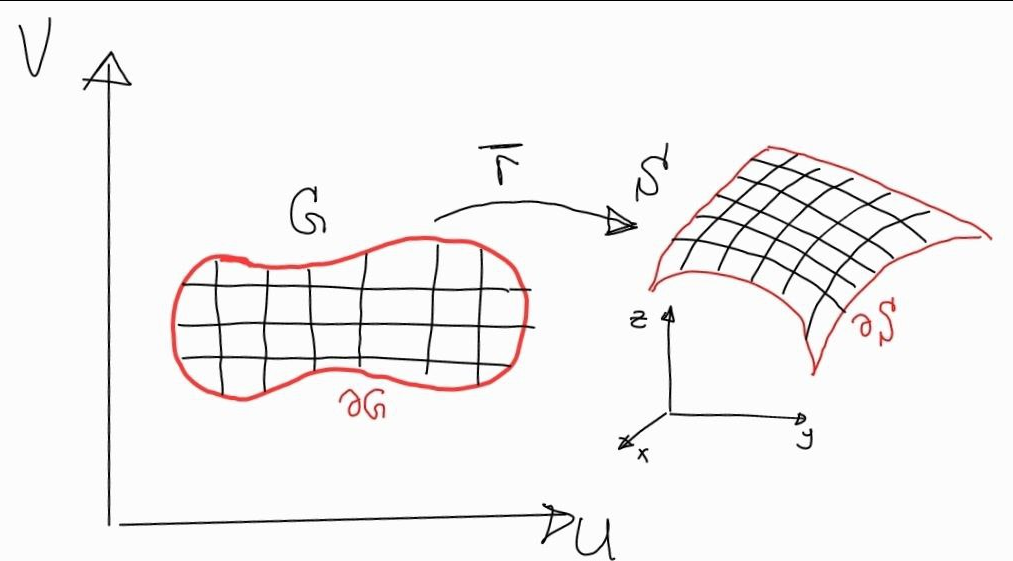
\includegraphics[width=\textwidth]{images/poverhnost.png}
\end{minipage}




\begin{definition}
    Будем говорить, что $S = \overline{r}(\overline{G})$~---~\textit{простая гладкая поверхность}, если:
    \begin{enumerate}
        \item[$\bullet$] $G$~---~область, граница которой является простым кусочно-гладким контуром (то есть замкнутая кривая без самопересечений кроме начала и конца, параметризация непрерывная и кусочно непрерывно дифференцируема и не имеет не более чем конечное число особых точек);
        \item[$\bullet$] $\overline{r}: \overline{G} \rightarrow S$~---~гомеоморфизм;
        \item[$\bullet$] $\overline{r} \in C^1(\overline{G}, \R^3)$;
        \item[$\bullet$] $[\overline{r}'_u \times \overline{r}'_v] \neq 0$ всюду на $\overline{G}$ (частные производные продолжаются на границу по непрерывности).
    \end{enumerate}
    Параметры $u, v$ можно рассматривать как внутренние координаты точек поверхности. Фиксируя одну из координат, мы получаем два семейства координатных кривых, покрывающих поверхность координатной сеткой.
\end{definition}
\begin{note}
    Верхняя половина сферы является простой гладкой поверхностью, а вот вся сфера уже не является простой гладкой поверхностью. Для этого придумали кусочно гладкую поверхность, см. далее
\end{note}
\begin{note}
    Будем называть касательной плоскостью к простой гладкой поверхности в точке $(u^0, v^0)$ линейную оболочку векторов $\overline{r}'_u(u^0, v^0)$ и $\overline{r}'_v(u^0, v^0)$~---~касательных векторов к координатным линиям. Вектором нормали в точке будем называть: \[ \overline{n}(\overline{r}(u_0, v_0)) := \frac{[\overline{r}'_u \times \overline{r}'_v]}{|[\overline{r}'_u \times \overline{r}'_v]|}.\]

\end{note}
\begin{definition}
    Пусть $\overline{r}: \overline{G} \rightarrow S$~---~отображение, удовлетворяющее условиям $1$) -- $4$) предыдущего определения. Будем говорить что $\overline{\rho}: \overline{\Omega} \rightarrow S$~---~допустимая параметризация, если $\exists \overline{F}: \overline{\Omega} \rightarrow \overline{G}$ ($\overline{\Omega} \subset\R^2_{\alpha, \beta} \text{, а } \overline{G} \subset \R^2_{u, v}$) всюду невырожденное такое, причём $J_F > 0$, что $\overline{\rho} = \overline{r} \circ \overline{F}$.
\end{definition}
\begin{reminder}
    (Дифференцируемость композиции функциий)
    Пусть $G \subset \R^n$~---~открыто и непусто, $\Omega \subset \R^m$~---~открыто и непусто. $F: G \rightarrow \Omega$ дифференцируемо в точке $x^0 \in G, H: \Omega \rightarrow \R^d$ дифференцируемо в точке $y^0 = F(x^0) \in \Omega$. Тогда для композиции $\phi = H \circ F$, якобиан будет равен: $J_\phi(x^0) = \D(H \circ F)(x^0) = \D H(F(x^0)) \D F(x^0)$, а $\frac{\partial \phi_i}{\partial x_j} = \sum \limits_{k = 1}^m \frac{\partial H_i}{\partial y_k} \cdot \frac{\partial F_k}{\partial x_j}, i \in \{1, \dots, d\}, j \in \{1, \dots, n\}$
\end{reminder}
\begin{lemma}
    Касательная плоскость и вектор нормали не зависят от выбора допустимой параметризации.
\end{lemma}
\begin{proof}
    Пусть $\overline{\rho}$ и $\overline{r}$~---~две допустимые параметризации. Тогда \[\overline{\rho}(\alpha, \beta) = \overline{r}(u(\alpha, \beta), v(\alpha, \beta)).\]
    Тогда по теореме о дифференцировании композиции:
    \begin{equation*}
    \begin{cases}
            \overline{\rho}'_\alpha = \overline{r}'_uu'_\alpha + \overline{r}'_vv'_\alpha \\
    \overline{\rho}'_\beta = \overline{r}'_uu'_\beta + \overline{r}'_vv'_\beta
    \end{cases}
    \biggr|\Rightarrow [\overline{\rho}'_\alpha \times \overline{\rho}'_\beta] = [\overline{r}'_u \times \overline{r}'_v] \cdot J_F (\alpha, \beta)
    \end{equation*}
    Где $F = (u, v)^T$~---~отображение репараметризации.
    Тогда вектора нормали коллинеарны и, следовательно, касательные плоскости совпадают.
\end{proof}
\begin{definition}
    Будем говорить что $S = \overline{r}(\overline{G})$~---~ поверхность~---~ориентируемая, если на ней существует непрерывное поле единичных нормалей, то есть существует $\overline{n}: S \rightarrow S^{\R^3}_1$: $\overline{n} \in C(S, S^2)$.
\end{definition}

\noindent 
\begin{minipage}{0.7\textwidth}
\begin{note}
    Не всякая поверхность ориентируема, например лента Мёбиуса. Далее с неориентируемыми поверхностями мы работать не будем.
\end{note}
\end{minipage}
\begin{minipage}{0.3\textwidth}
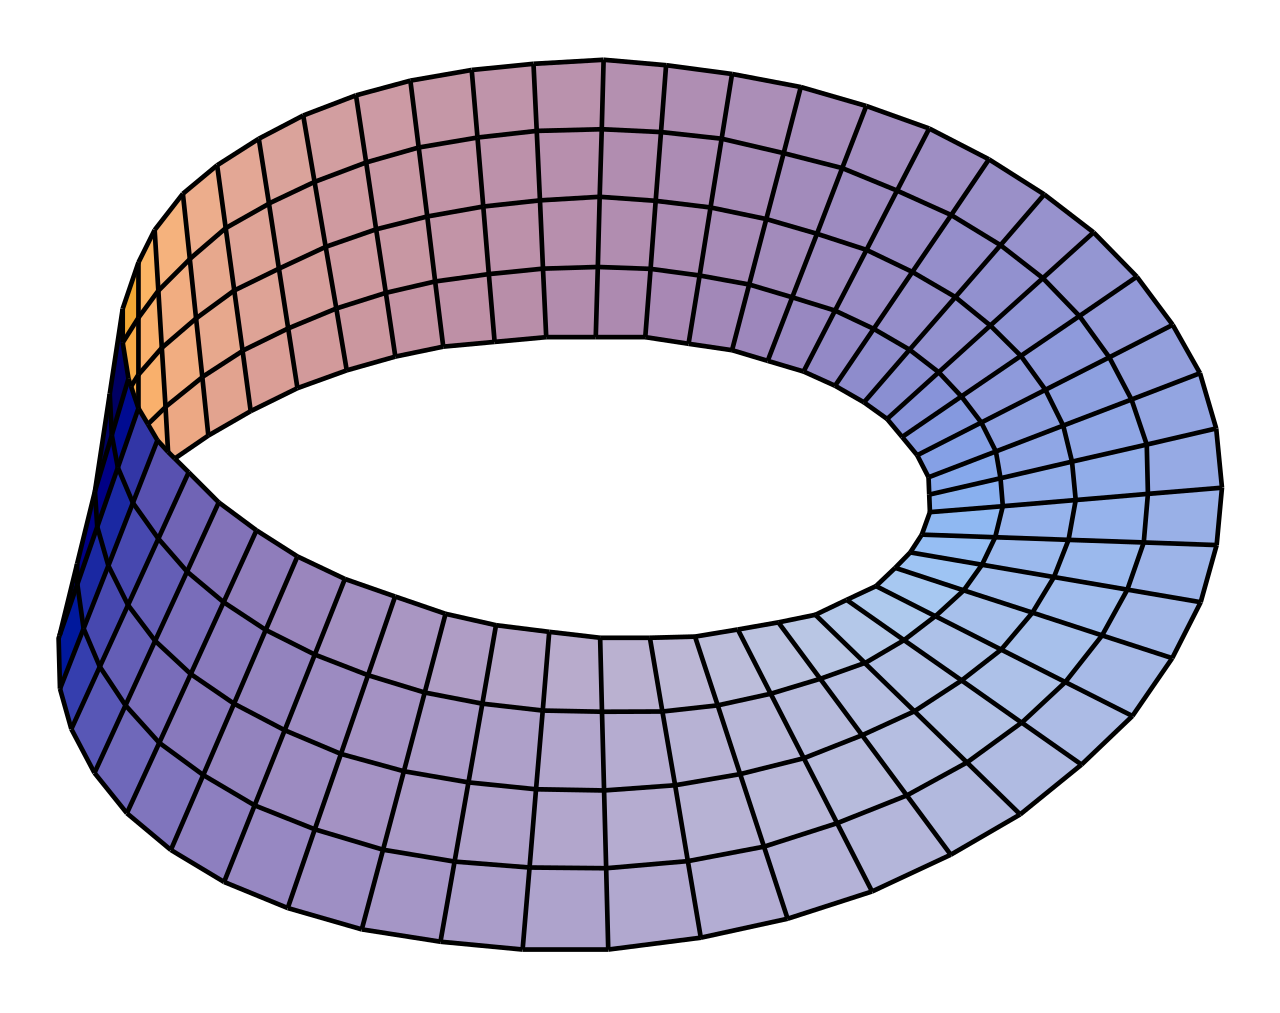
\includegraphics[width=\textwidth]{images/mebius.png}
\end{minipage}


\begin{note}
    Всякая простая гладкая поверхность ориентируема, причём она имеет ровно две ориентации, которые задаются как \[\overline{n}_\pm = \pm \dfrac{[\overline{r}'_u \times \overline{r}'_v]}{|[\overline{r}'_u \times \overline{r}'_v]|}.\]
\end{note}
\begin{corollary}
    Ориентация простой гладкой поверхности не зависит от выбора допустимой параметризации.
\end{corollary}

\noindent 
\begin{minipage}{0.6\textwidth}
\begin{definition}[Ориентация края]
    Пусть есть простая гладкая (а значит ориентируемая) поверхность $S$ с допустимой параметризацией $\overline{r}: \overline{G} \rightarrow \R^3$. Пусть $\partial  G = \{\rho(t) \mid t \in [t_1, t_2]\}$~---~простой кусочно-гладкий контур; $\overline{v} = \overline{\rho}'(t) \neq 0$. По определению, $\partial  S = \overline{r}(\partial G)$. Тогда касательный вектор $\overline{\tau}$ к краю $\partial S$: \[\overline{\tau}(t_0) = \dfrac{d}{dt}\overline{r}(\overline{\rho(t)})|_{t = t_0} = \overline{r}'_u \Big(u(t_0), v(t_0)\Big)u'(t_0) + \overline{r}'_v \Big(u(t_0), v(t_0) \Big)v'(t_0)\]
    Пусть \[\overline{\xi}(h) = \rho(t_0) + h\overline{n}(t_0),\]
    
\end{definition}
\end{minipage}
\begin{minipage}{0.4\textwidth}
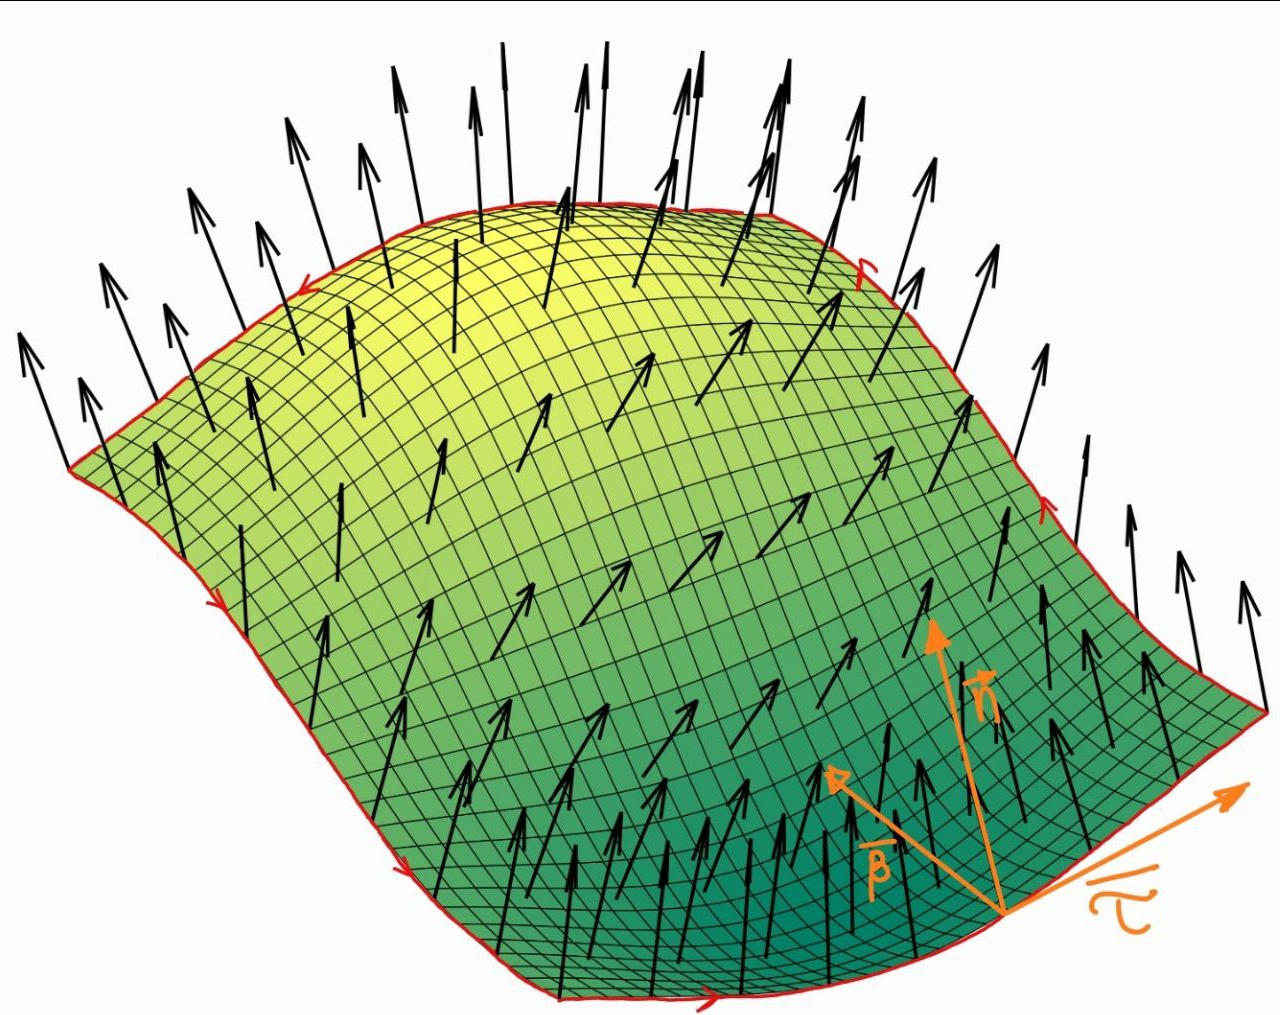
\includegraphics[width=\textwidth]{images/pov_orientation.png}
\end{minipage}
где $\overline{n}$~---~вектор внутренней нормали. Тогда введём вектор $\overline{\beta}$ как \[\beta(t_0) = (\overline{r} \circ \overline{\xi})'_h|_{h = 0} = \overline{r}'_un_u + \overline{r}'_vn_v.\]
\begin{definition}
    Будем говорить, что край $\partial S$ простой гладкой поверхности ориентирован относительно неё положительно, если в любой точке гладкости края тройка векторов $(\overline{\tau}, \overline{\beta}, \overline{n})$~---~правая. Неформально, у нас есть поле нормалей поверхностей, обходя край, область будет слева

\end{definition}
    
\begin{lemma}[Достаточное условие ориентируемости края поверхности]
Пусть заданы правые базисы в $\R^2_{uv}$ и $\R^3_{xyz}$. Пусть $\partial G$ положительно ориентирована относительно области $G$.\begin{enumerate}
    \item Пусть $S = \overline{r}(\overline{G})$~---~простая гладкая поверхность;
    \item $\partial S$ ориентирован согласованно с ориентацией $\partial G$;
    \item Пусть $S$ ориентирована полем $\overline{n} = \frac{\overline{r}'_u \times \overline{r}'_v}{|\overline{r}'_u \times \overline{r}'_v|}$.
\end{enumerate}  
    Тогда $\partial S$ ориентирован положительно относительно $S$. (Если нарушить только условие 2 или 3, то будет отрицательно ориентирован, а если оба сразу, то положительно)
\end{lemma}
\begin{proof}
    Из условия правости базиса на поверхности следует, что если $\rho(t_0)$~---~точка гладкости границы $G$, то $\overline{v}, \overline{N}$~---~правая двойка, то есть \[
        \det \begin{pmatrix}
            u'(t_0) & N_u \\ v'(t_0) & N_v
        \end{pmatrix} > 0.
    \]
    Касательный вектор к поверхности записывается как \[\overline{\tau}(t_0) = \dfrac{d}{dt} \overline{r}(u(t), v(t))|_{t = t_0} = \overline{r}'_u \Big(u(t_0), v(t_0)\Big)u'(t_0) + \overline{r}'_v \Big(u(t_0), v(t_0) \Big)v'(t_0)\]
    А вектор бинормали как \[\overline{\beta}(t_0) = \dfrac{d}{dt} \overline{r}(t_0 + \overline{N}t)|_{t = 0} = \overline{r}'_u \Big(u(t_0), v(t_0)\Big)N_u + \overline{r}'_v \Big(u(t_0), v(t_0)\Big)N_v\]
    Тогда \[ [\overline{\tau}(t_0) \times \overline{\beta}(t_0)] = [\overline{r}'_u \times \overline{r}'_v] \cdot \begin{vmatrix}
        u'(t_0) & N_u \\ v'(t_0) & N_v
    \end{vmatrix}\]
    Значит $\overline{\tau} \times \overline{\beta}$ коллинеарен нормали и $\overline{\tau}, \overline{\beta}, \overline{n}$~---~правая тройка.
\end{proof}
\begin{definition}
    Будем говорить, что $S$~---~кусочно-гладкая поверхность, если:
    \begin{itemize}
        \item $S = \bigcup\limits_{i = 1}^N S_i$, где каждая из $S_i$~---~простая гладкая поверхность
        \item $S_i \cap S_j = \partial S_i \cap \partial S_j$ для всяких двух $i$ и $j$.
        \item $\partial S_i \cap \partial S_j$~---~либо состоит из конечного числа точек, либо пусто, либо состоит из конечного числа простых кусочно-гладких кривых (и, быть может, конечного числа точек). Будем называть два куска соседними, если они пересекаются по кусочно-гладкой кривой.
        \item Для $\forall i, j, k: i \neq j, i \neq k, j \neq k$ выполнено, что $\partial S_i \cap \partial S_j \cap \partial S_k$  состоит из не более чем конечного числа точек.
        \item $\forall i \neq j$ существует конечный набор $S_i = S_{k_1}, \ldots, S_{k_s} = S_j$ т.ч. $S_{k_r}$ и $S_{k_{r + 1}}$~---~соседние для всех $r$.
    \end{itemize}
\end{definition}
\begin{example}
    Это определение это естественное обобщение многогранников. Примеры кусочно гладких поверхностей: сфера, конус, пирамида. Пример не кусочно гладкой поверхности это два конуса, которые стоят вертикально, но касаются основаниями в одной точке
\end{example}
\begin{definition}
    Пусть есть кусочно-гладкая поверхность $S = \bigcup\limits_{ i = 1}^N S_i$. Для каждого куска поверхности определим внешнюю часть границы следующим образом: $\partial^eS_i$~---~все такие точки, т.ч. они лежат только на $\partial S_i$, то есть $\forall j \neq i \hookleftarrow \partial^e S_i \cap \partial S_j = \emptyset$, а внутреннюю -- как все остальные точки границы. Пусть ориентация $\partial S_j$ выбрана так, что если $S_i$ и $S_j$~---~соседние, то $\partial S_i \cap \partial S_j$~---~то положительная ориентация кривой относительно $S_i$ соответствует отрицательной ориентации кривой относительно $S_j$, т.е. ориентации согласованы.
    Тогда будем говорить, что $\partial S = \bigcup\limits_{i = 1}^N \partial^e S_i \cup A$, где $A$~---~конечное множество точек ориентирован, и его ориентация соответствует ориентации $\partial^eS_i$.
\end{definition}

\begin{definition}
    Край кусочно-гладкой поверхности $S$ называется ориентированным согласовано с ориентацией $S$, если $\forall i$ край $S_i$ ориентирован согласованно с ориентацией $S$.
\end{definition}

\subsection{Поверхностные интегралы I рода}
Физический смысл --- это вычисление массы тела с распределением плотности $f(\overline{r})$.
\begin{definition}
    Пусть $S = \overline{r}(\overline{G})$~---~простая гладкая поверхность. Пусть $f$: $S \rightarrow \R$: $f \in C(S, \R)$. Тогда \textit{поверхностным интегралом первого рода} будем называть \[\iint\limits_S f(\overline{r})ds := \iint\limits_G f(\overline{r}(u, v))|[\overline{r}'_u \times \overline{r}'_v]|dudv.\]
\end{definition}
\begin{definition}
    \textit{Площадью} простой гладкой поверхности будем по определению называть \[\iint\limits_S 1ds = \iint\limits_G |[\overline{r}'_u \times \overline{r}'_v]|dudv.\]
\end{definition}
%где был че виедл
%на сфере, диффеоморфизмы
%ахуй
%:)